\begin{frame}{Patch Embedding}
    \begin{itemize}
        \item \textbf{Patch Embedding:} Achieved via a linear projection of flattened patches (\(P=16\) typical)
        \item \textbf{Differences from CNN stems:}
        \begin{itemize}
            \item Large stride causes optimization instability
            \item Mitigated via convolutional preprocessing (e.g., small conv stem)
        \end{itemize}
    \end{itemize}
\end{frame}

\begin{frame}{ViT: Learning Patterns}
    \begin{figure}
        \centering
        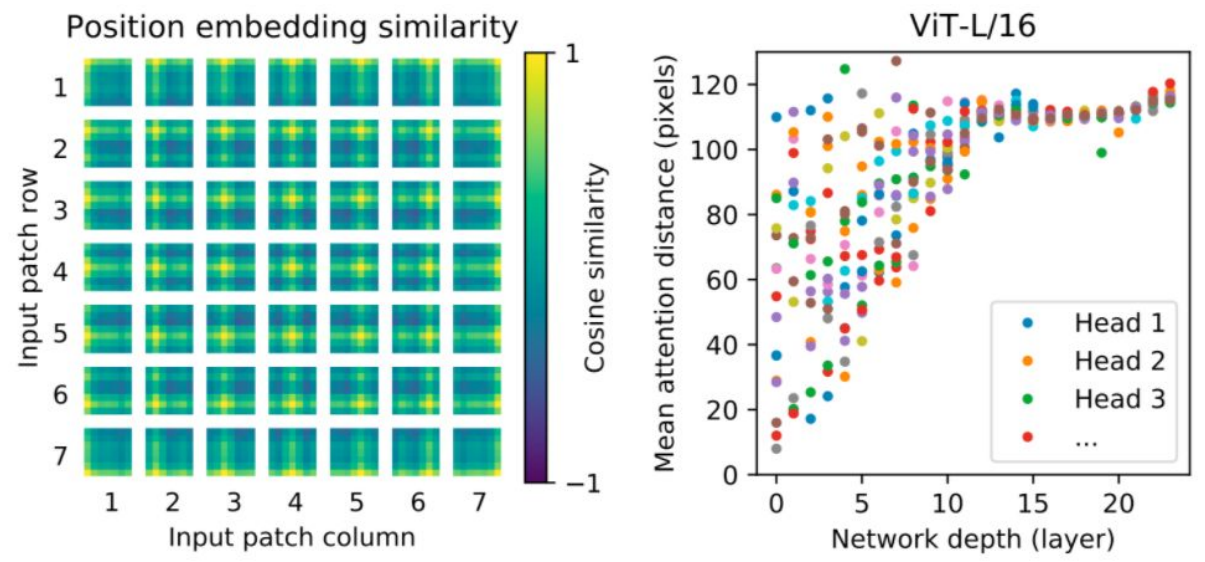
\includegraphics[width=0.85\linewidth,height=\textheight,keepaspectratio]{images/vit/learning_patterns.png}
    \end{figure}
    \begin{itemize}
        \item ViT learns the grid-like structure of the image patches via its position embeddings.
        \item The lower layers contain both global and local features, while the higher layers contain only global features.
    \end{itemize}
\end{frame}